% Compile from this directory: xelatex -interaction=nonstopmode final.tex (twice).
% Figures in final_assets/ are rebuilt by build_final_figures.py from saved CSV/JSON.
% Main evidence: final_technical_report.md/.pdf; selected history: prev_report.pdf.
\documentclass[11pt,a4paper]{article}
\usepackage{fontspec}
\setmainfont{Times New Roman}
\setsansfont{Arial}
\setmonofont{Consolas}[Scale=0.88]
\usepackage[top=20.32mm,bottom=17.78mm,left=17.78mm,right=17.78mm,headheight=12pt,headsep=7mm,footskip=10mm]{geometry}
\usepackage{setspace,graphicx,booktabs,tabularx,array,enumitem,amsmath,fix-cm,xcolor,tikz,caption,fancyhdr,titlesec,needspace}
\usetikzlibrary{arrows.meta,positioning,calc}
\usepackage[hidelinks]{hyperref}
\usepackage{xurl}
\graphicspath{{final_assets/}{plots/}}
\setstretch{1.15}
\setlength{\parindent}{0pt}
\setlength{\parskip}{6pt}
\setlength{\emergencystretch}{2em}
\pagestyle{fancy}\fancyhf{}
\rhead{\sffamily\fontsize{8.5}{10}\selectfont CSE 4112: Machine Learning Laboratory | Dataset Report}
\cfoot{\thepage}\renewcommand{\headrulewidth}{0pt}
\titleformat{\section}{\sffamily\fontsize{13}{15}\selectfont\bfseries}{\thesection.}{.5em}{}
\titleformat{\subsection}{\sffamily\fontsize{11.5}{13.5}\selectfont\bfseries}{\thesubsection}{.5em}{}
\titlespacing*{\section}{0pt}{8pt}{4pt}
\titlespacing*{\subsection}{0pt}{5pt}{4pt}
\captionsetup{font={small,stretch=1},labelfont=bf,skip=5pt,hypcap=false}
\setlist{leftmargin=5mm,itemsep=2pt,topsep=3pt,parsep=0pt}
\newcolumntype{L}[1]{>{\raggedright\arraybackslash}p{#1}}
\newcolumntype{Y}{>{\raggedright\arraybackslash}X}
\newcommand{\code}[1]{\texttt{#1}}
\newcommand{\datasetlink}{\href{https://drive.google.com/drive/u/1/folders/1XN55OGpozy5Rhbs5QRFMatlCMTAo8sPu}{Dataset folder on Google Drive}}
\newcommand{\codeurl}{\url{https://github.com/MishtiAloo/ML-train.git}}
\newcommand{\cont}[1]{\par{\sffamily\bfseries #1}\par}
\newenvironment{datatable}[2]{\begin{center}\begin{minipage}{\linewidth}\setstretch{1}\small\captionof{table}{#1}\label{#2}\vspace{2pt}\renewcommand{\arraystretch}{1.18}}{\end{minipage}\end{center}}
\newcommand{\fig}[4]{\begin{center}\includegraphics[width=#2\linewidth]{#1}\captionof{figure}{#3}\label{#4}\end{center}}
\newcommand{\nextpage}{\clearpage}
\definecolor{input}{HTML}{DCECF4}
\definecolor{frozen}{HTML}{E7E7E7}
\definecolor{train}{HTML}{E8DCF0}
\definecolor{out}{HTML}{E0EEDD}
\definecolor{validation}{HTML}{F3DB83}
\definecolor{rejected}{HTML}{E4A3A0}
\tikzset{box/.style={draw=black!75,rounded corners=2pt,align=center,text width=45mm,minimum height=13mm,inner sep=5pt,font=\sffamily\fontsize{10.5}{12}\selectfont},arrow/.style={-{Latex[length=2mm]},thick},lab/.style={font=\sffamily\fontsize{10}{11}\selectfont,fill=white,inner sep=2pt}}
\hypersetup{pdftitle={Occlusion-Robust Face Identification Dataset: ArcFace Evaluation},pdfauthor={CSE 4112, KUET; rolls 2107031, 2107044, 2107046, 2107047, 2107057, 2107059}}
\begin{document}

% PAGE 1: visual synopsis required by the supplied template.
\begin{center}
{\sffamily\fontsize{13}{15}\selectfont\bfseries Khulna University of Engineering \& Technology\par}
{\fontsize{13}{15}\selectfont Department of Computer Science and Engineering\par}
{\sffamily\fontsize{13}{15}\selectfont\bfseries CSE 4112: Machine Learning Laboratory\par}
\vspace{3mm}
{\sffamily\fontsize{20}{23}\selectfont\bfseries DATASET REPORT\par}
{\fontsize{13.5}{16}\selectfont\bfseries\itshape Occlusion-Robust Face Identification Dataset:\\Evaluation with a Partially Fine-Tuned ArcFace Model\par}
\end{center}
\begin{datatable}{Submission and dataset identification.}{tab:cover}
\begin{tabularx}{\linewidth}{L{26mm}Y L{28mm}Y}\toprule
Group No. & 5 & Dataset version & 1\\
Students & \multicolumn{3}{p{139mm}}{Adiba Tahsin (2107031), Arafat Islam (2107044), Arman Rahman Rafi (2107046), Dip Shekhor Datta (2107047), Megha Tania (2107057), Farhan Tahmid (2107059)}\\
Submission date & \multicolumn{3}{l}{22/09/2026}\\
Repository & \multicolumn{3}{p{139mm}}{\url{https://drive.google.com/drive/u/1/folders/1XN55OGpozy5Rhbs5QRFMatlCMTAo8sPu}}\\\bottomrule
\end{tabularx}
\end{datatable}
\cont{(a) Framework illustrating the practical application of the data}
\begin{center}
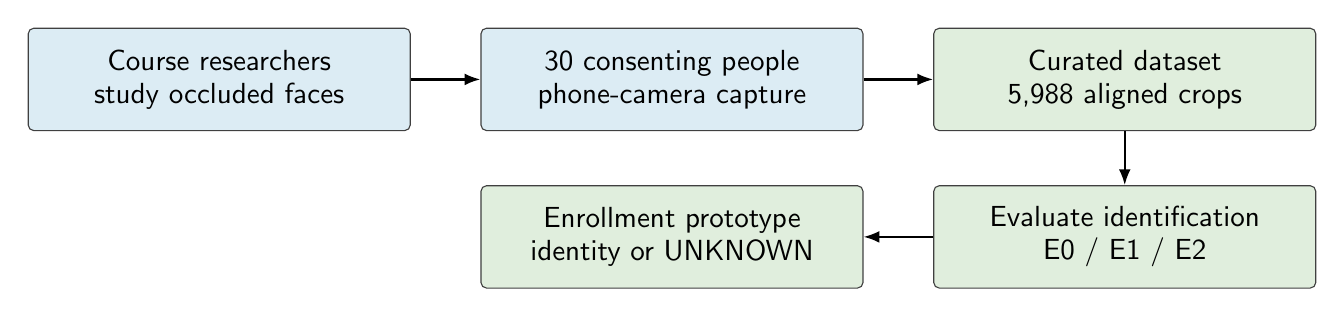
\begin{tikzpicture}
\node[box,fill=input] (a) at (0,0) {Course researchers\\study occluded faces};
\node[box,fill=input] (b) at (5.75,0) {30 consenting people\\phone-camera capture};
\node[box,fill=out] (c) at (11.5,0) {Curated dataset\\5,988 aligned crops};
\node[box,fill=out] (d) at (11.5,-2) {Evaluate identification\\E0 / E1 / E2};
\node[box,fill=out] (e) at (5.75,-2) {Enrollment prototype\\identity or UNKNOWN};
\draw[arrow](a)--(b);\draw[arrow](b)--(c);\draw[arrow](c)--(d);\draw[arrow](d)--(e);
\end{tikzpicture}
\renewcommand{\thefigure}{1(a)}
\captionof{figure}{Practical use: an academic enrollment study of recognition under occlusion. The output supports robustness analysis and prototype decisions.}
\label{fig:application}
\end{center}
\cont{(b) Technical pipeline of the ML method using the dataset}
\begin{center}
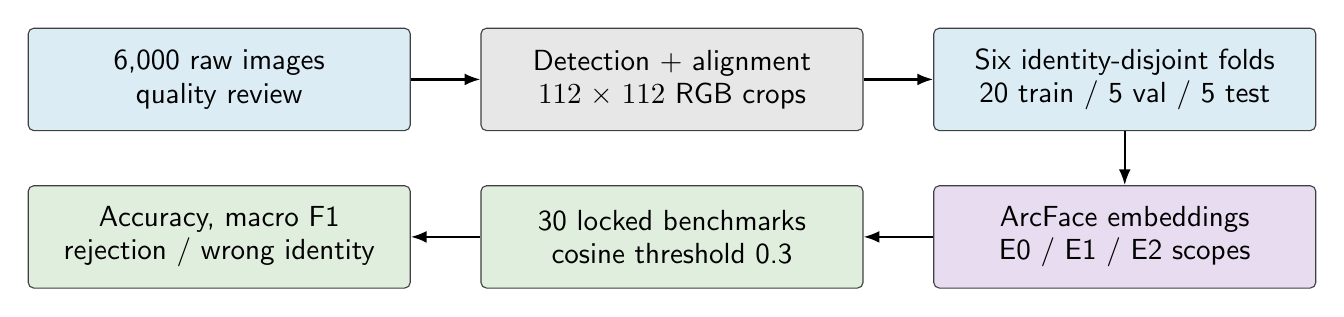
\begin{tikzpicture}
\node[box,fill=input] (a) at (0,0) {6,000 raw images\\quality review};
\node[box,fill=frozen] (b) at (5.75,0) {Detection + alignment\\$112\times112$ RGB crops};
\node[box,fill=input] (c) at (11.5,0) {Six identity-disjoint folds\\20 train / 5 val / 5 test};
\node[box,fill=train] (d) at (11.5,-2) {ArcFace embeddings\\E0 / E1 / E2 scopes};
\node[box,fill=out] (e) at (5.75,-2) {30 locked benchmarks\\cosine threshold 0.3};
\node[box,fill=out] (f) at (0,-2) {Accuracy, macro F1\\rejection / wrong identity};
\draw[arrow](a)--(b);\draw[arrow](b)--(c);\draw[arrow](c)--(d);\draw[arrow](d)--(e);\draw[arrow](e)--(f);
\end{tikzpicture}
\addtocounter{figure}{-1}
\renewcommand{\thefigure}{1(b)}
\captionof{figure}{Technical synopsis. Benchmark photographs and burst neighbours are excluded from queries; augmentation is applied only to training images.}
\label{fig:synopsis}
\renewcommand{\thefigure}{\arabic{figure}}
\end{center}
\vfill
{\small\textbf{Submitted to:} Dr. Muhammad Aminul Haque Akhand, Professor; Nabil Faiyaz Sadi, Lecturer, Department of CSE.\par
\textbf{Submitted by:} the six students in Table~\ref{tab:cover}; Section A, Year 4, Semester 1.\par
\centering Khulna-9203, Bangladesh\par}

% PAGE 2
\nextpage
\section{Dataset Article Information}
Table~\ref{tab:article} identifies the dataset and its documented access status.
\begin{datatable}{Dataset article information. Missing administrative facts are stated explicitly.}{tab:article}
\begin{tabularx}{\linewidth}{L{40mm}Y}\toprule
Dataset/report title & Occlusion-Robust Face Identification Dataset: Evaluation with a Partially Fine-Tuned ArcFace Model\\
Group and students & Group 5: Adiba Tahsin (2107031), Arafat Islam (2107044), Arman Rahman Rafi (2107046), Dip Shekhor Datta (2107047), Megha Tania (2107057), Farhan Tahmid (2107059).\\
Affiliation & Department of Computer Science and Engineering, KUET, Khulna-9203, Bangladesh\\
Student emails & \nolinkurl{tahsin2107031@stud.kuet.ac.bd}; \nolinkurl{islam2107044@stud.kuet.ac.bd}; \nolinkurl{rafi2107046@stud.kuet.ac.bd}; \nolinkurl{datta2107047@stud.kuet.ac.bd}; \nolinkurl{tania2107057@stud.kuet.ac.bd}; \nolinkurl{tahmid2107059@stud.kuet.ac.bd}\\
Corresponding student & Not supplied\\
Keywords & Facial occlusion; enrollment; person-disjoint evaluation; angular-margin learning; benchmark embeddings; dataset curation\\
Dataset version & 1; submission date: 22/09/2026; release date: not supplied\\
Repository / persistent ID & \datasetlink\\
License & Restricted academic use under participant consent; no public redistribution license documented\\
Related article / source & Primary project collection; final technical report is the authoritative experiment record. Related published work is discussed in Section 5.\\\bottomrule
\end{tabularx}
\end{datatable}
\section{Abstract}
This dataset was created to study face identification when masks, glasses, scarves, caps, and combinations of coverings hide identity-bearing facial regions. Six students recruited 30 consenting participants and collected 6,000 phone-camera photographs in indoor regular and low lighting. The collection covers eight occlusion labels, with natural head-pose variation during capture. A fixed face-detection and five-landmark alignment pipeline produced 5,988 RGB face crops of $112\times112$ pixels. Twelve photographs did not yield detectable faces and are excluded from the recognition dataset. Image files are accompanied by a CSV manifest containing pseudonymous participant identifiers, occlusion and lighting labels, source references, hashes, grouping information, and detector-quality fields.

The data package supports reproducible enrollment-style identification experiments with pretrained ArcFace embeddings. A six-fold protocol assigns complete identities to training, validation, and testing, while a single clean benchmark per participant provides the enrollment gallery. Benchmark images and their near-duplicate burst neighbours are excluded from queries. Saved fold definitions, checkpoints, predictions, confusion matrices, and training histories support reuse for studying occlusion sensitivity, rejection behaviour, and the transfer of partial fine-tuning to unseen identities. Quality documentation distinguishes capture review, detection failure, coverage imbalance, and retained duplicates. Access remains restricted because facial images are identifiable; participant codes do not make the photographs anonymous. Reuse should preserve consent conditions, identity-level partitioning, and the distinction between detector success and recognition performance.

% PAGE 3
\nextpage
\section{Dataset Specifications Table}
Table~\ref{tab:spec} summarizes the collection and its reusable records.
\begin{datatable}{Dataset specifications.}{tab:spec}
\begin{tabularx}{\linewidth}{L{40mm}Y}\toprule
Item & Required information\\\midrule
Subject / domain & Computer vision; biometric pattern recognition\\
Specific subject area & Identification of enrolled people under single and combined facial occlusions\\
Type of data & Primary facial photographs, aligned crops, metadata, and derived experiment records\\
File formats & JPEG images; CSV manifest and confusion matrices; JSON fold definitions and metrics; NPZ benchmark embeddings; PT checkpoints; ONNX pretrained models\\
Unit of observation & One face photograph / aligned crop linked to one participant and one occlusion--lighting condition\\
Data collection / source & Primary phone-camera collection by six team members; convenience sample of themselves and consenting relatives/acquaintances\\
Instrument / software & Phone cameras (models: not supplied); InsightFace \code{buffalo\_l}; RetinaFace \code{det\_10g.onnx}; ArcFace \code{w600k\_r50.onnx}; PyTorch, ONNX Runtime and onnx2torch (versions: not supplied)\\
Data source location & Indoor capture; KUET-affiliated project, Bangladesh. Exact capture sites: not supplied.\\
Collection period & Start/end dates: not supplied\\
Dataset size & 30 identities; 6,000 raw photographs; 5,988 aligned crops; 8 occlusion categories; 2 lighting labels; 5,818 pooled evaluation queries\\
Target / labels & Pseudonymous identity \code{p01}--\code{p30}; occlusion and lighting are condition labels\\
Accessibility & \datasetlink; access is governed by the folder's sharing permissions and participant consent\\
License / reuse terms & Academic, non-commercial consent; raw images and identity mapping restricted to the six members; recognizable report/demo images require separate optional consent\\\bottomrule
\end{tabularx}
\end{datatable}
\section{Value of the Data}
\begin{itemize}
\item Eight covering conditions support comparisons of eye-region, lower-face, and combined occlusion within one enrollment task.
\item Aligned crops and detector-quality metadata let students study recognition errors separately from failures of face detection.
\item Identity-level folds support measuring whether adaptation on 20 people transfers to different enrolled identities.
\item Fixed benchmarks and recorded exclusions permit reproducible evaluation without query--gallery burst overlap.
\item Saved predictions and histories support rejection analysis, per-person metrics, and comparisons of limited fine-tuning scopes.
\end{itemize}

% PAGE 4
\nextpage
\section{Background and Practical Motivation}
\cont{Introduction and objective}
Face identification becomes difficult when a covering removes the features used to distinguish one person from another. Masks hide the nose, mouth and jawline; sunglasses hide the eyes; a cap changes the visible forehead region. Combining a mask with sunglasses removes both major regions at once. Dim illumination and head tilt can further reduce the information available to detection and recognition. The practical framework in Figure~\ref{fig:application} therefore begins with a controlled collection of consented examples and ends with an enrollment prototype that can return either a participant identifier or UNKNOWN.

The intended users are course researchers and students testing the reliability of a small face-identification system. All query identities are enrolled, but test identities are absent from fine-tuning. This distinguishes transfer to new people from memorization of training identities. The technical pipeline in Figure~\ref{fig:synopsis} makes this distinction explicit: whole people are assigned to folds, while clean enrollment benchmarks are available for all 30 identities.

Existing work provides complementary precedents. Pgu-Face is a controlled partially covered-face dataset with more participants but fewer images per participant and narrower covering variation~\cite{pgu}. Chong et al. study masked-face recognition with CNN features and an SVM~\cite{chong}. Montero et al. adapt ArcFace to masked faces through a multi-task approach~\cite{montero}. Table~\ref{tab:related} relates these works to the present collection. Their results cannot be ranked directly against this project's accuracies because datasets, identity counts and evaluation protocols differ.

The present experiment asks how much occlusion a pretrained representation already tolerates and whether a restricted update improves transfer to unseen identities. Its contribution is a documented local dataset and reproducible comparison, rather than a claim of a new recognition algorithm or population-wide biometric reliability.
\begin{datatable}{Related/base papers retained from the previous report, interpreted under the final evaluation protocol.}{tab:related}
\begin{tabularx}{\linewidth}{L{35mm}Y Y}\toprule
Paper & Contribution & Relation to this report\\\midrule
Salari and Rostami (2016)~\cite{pgu} & Pgu-Face: 896 images of 224 subjects, four images per subject, with facial-hair and sunglasses variation. & Capture/dataset precedent; the local collection has more images and covering categories but fewer identities.\\
Chong, Chong and Ong (2022)~\cite{chong} & CNN feature extraction with SVM classification on masked-face benchmarks. & Recognition-method precedent; this study uses pretrained ArcFace embeddings and fixed benchmark matching.\\
Montero et al. (2022)~\cite{montero} & Multi-task ArcFace approach combining identity recognition and mask-related training. & ArcFace-family precedent; this study changes the trainable scope without adding a mask-detection objective.\\\bottomrule
\end{tabularx}
\end{datatable}

% PAGE 5
\nextpage
\section{Data Acquisition / Experimental Design, Materials and Methods}
\subsection{Data source and sampling strategy}
Thirty identities (\code{p01}--\code{p30}) were enrolled. Each of six team members recruited, photographed and annotated five people: themselves and four consenting relatives or acquaintances. This is a convenience sample, not a representative demographic sample. The participant-to-photographer mapping was kept internally in \path{metadata/person_id_mapping.txt}, as described in the previous report. The age distribution is 26 participants aged 23--24 years and one each aged 28, 39, 44 and 78 years.
\subsection{Collection setting, period and location}
Each participant was photographed in one sitting under regular and low indoor illumination, using a phone camera. The capture plan targeted 200 images per participant, totaling 6,000 images. Exact sites, acquisition dates, camera distances and exposure settings: not supplied. Head positions varied naturally rather than through a logged per-image pose label.
\subsection{Instruments, hardware, software and versions}
Phone camera models and capture-app versions: not supplied. Preprocessing uses the project's RetinaFace detection and five-landmark alignment stage, \code{det\_10g.onnx}, within InsightFace's \code{buffalo\_l} package. Recognition uses \code{w600k\_r50.onnx} (IResNet-50). ONNX Runtime, onnx2torch and PyTorch support conversion and fine-tuning. The training record describes an RTX 3090 machine; exact package versions: not supplied.
\subsection{Variables, measurements and metadata}
Recorded fields include participant identity, occlusion, lighting, source/crop paths, source stem, MD5, burst group, detector status, confidence and bounding-box area fraction. Table~\ref{tab:conditions} defines the capture categories. Detector confidence is a model score, not a calibrated probability of image quality.
\begin{datatable}{Capture categories. Only lighting and covering are recorded as per-image condition labels.}{tab:conditions}
\begin{tabularx}{\linewidth}{L{29mm}Y}\toprule
Dimension & Labels and interpretation\\\midrule
Informal pose & Front; left/right head turn; up/down chin tilt. Encouraged during capture, not recorded per image.\\
Lighting & \code{regular}: ordinary indoor illumination; \code{low}: dimmer indoor capture\\
Single / no covering & \code{none}, \code{mask}, \code{sunglass}, \code{clearglass}, \code{scarf}, \code{cap}\\
Combined covering & \code{mask\_sunglass}, \code{mask\_clearglass}\\\bottomrule
\end{tabularx}
\end{datatable}
\subsection{Annotation / labeling protocol}
Capture filenames encode identity, occlusion and lighting, for example \code{p07\_mask\_sunglass\_low\_014.jpg}. The manifest is the authoritative metadata source. Each student annotated their own five participants' data. Labels describe known capture conditions, and inter-rater agreement checking was completed. Agreement method, coefficient and adjudication details: not supplied.
\subsection{Provenance, versioning and raw-data preservation}
The previous report describes retaining rejected photographs in \code{put\_asides/}, with reasons, and freezing the accepted capture set before training. The final records link raw files to crops and source stems and retain hashes. Dataset version 1 is documented for the 22/09/2026 submission; the documentation revision is recorded in \path{docs/FINAL_README.txt}. Paths recorded on the training machine must be remapped when the project is moved.

% PAGE 6
\nextpage
\section{Data Description / Data Records}
\subsection{Repository / Folder Structure}
Table~\ref{tab:files} describes the project layout. Paths are relative to the project root unless marked otherwise; the raw-image directory is a sibling of that root.
\begin{datatable}{Data and experiment records. Fold denotes one of six identity rotations; exp is e0, e1 or e2.}{tab:files}
\begin{tabularx}{\linewidth}{L{69mm}Y L{23mm}}\toprule
Folder / file & Contents & Record type\\\midrule
\path{../processed_data/} & Original capture set used for preprocessing; named in source scripts & Raw\\
\path{crops/} & 5,988 aligned face images, organized by person & Processed\\
\path{metadata/manifest.csv} & Image labels, provenance and quality fields & Metadata\\
\path{metadata/e1e2_person_folds.json} & Train/validation/test people, benchmark photos and exclusions & Metadata\\
\path{runs/e1e2/person_benchmarks.npz} & 30 locked 512-dimensional gallery embeddings & Derived\\
\path{runs/e1e2/folds/fold*/} & Selected models, epoch histories and test-result JSON files & Experiment\\
\path{runs/e1e2/analysis/} & Predictions, 30$\times$31 confusion CSVs and metric JSON files & Analysis\\
\path{runs/e1e2/learning_curve/} & Repeated runs with validation gallery loss added & Analysis\\
\path{runs/e1e2/learning_curve_matched/} & Repeated runs scoring training and validation people with one common loss & Analysis\\
\path{models/}; \path{scripts/} & Pretrained ONNX models; preparation, training and analysis scripts & Software\\
\path{docs/} & Technical reports, metric tables, plots and this report & Documentation\\\bottomrule
\end{tabularx}
\end{datatable}
\subsection{Data Dictionary}
Table~\ref{tab:dictionary} defines the principal fields. The remaining provenance and processing fields appear in Appendix A. All 13 columns are non-empty in the supplied manifest; this does not prove the labels or provenance are error-free.
\begin{datatable}{Principal manifest fields. Missing-value rule: required values should be checked; no missing values occur in this snapshot.}{tab:dictionary}
\begin{tabularx}{\linewidth}{L{27mm}Y L{14mm}L{19mm}L{31mm}L{19mm}}\toprule
Variable & Meaning & Type & Unit/range & Coding & Missing rule\\\midrule
\code{person\_id} & Participant label & Text & 30 IDs & p01--p30 & Required\\
\code{occlusion} & Covering condition & Text & 8 classes & Table~\ref{tab:conditions} & Required\\
\code{lighting} & Lighting condition & Text & 2 classes & regular / low & Required\\
\code{det\_score} & Detector confidence & Float & $[0,1]$ & Numeric score & Required\\
\code{bbox\_area\_frac} & Box/image area ratio & Float & $[0,1]$ & Unitless & Required\\
\code{group\_id} & Related-frame group & Text & Identifier & e.g. g0 & Required\\\bottomrule
\end{tabularx}
\end{datatable}
\textbf{Partition warning.} The manifest contains a legacy \code{split} field. The final experiments instead use \path{e1e2_person_folds.json}. Treating the legacy field as the final protocol would change the evaluation.

% PAGE 7
\nextpage
\subsection{Dataset Composition and Descriptive Overview}
The manifest contains 5,988 crops from 30 people: 3,050 under regular lighting and 2,938 under low lighting. Figure~\ref{fig:composition} shows the retained category counts. Scarf coverage is narrower: only 24 of the 30 people have that condition, and the final technical report notes two further person--condition gaps. The target capture plan therefore does not imply a fully balanced realized dataset.
\fig{composition.pdf}{1}{Retained images by occlusion, before benchmark/query exclusions. The 837 unoccluded images become 667 evaluation queries after 170 benchmark and related-frame exclusions.}{fig:composition}
The examples in Figure~\ref{fig:samples} show how alignment standardizes model input while preserving different visible face regions. All inputs have the same spatial size; occlusion remains part of the task.
\fig{samples.pdf}{1}{Participant p11 across all eight covering conditions: raw photographs followed by their corresponding aligned crops. The $112\times112$ aligned face is the input to ArcFace.}{fig:samples}

% PAGE 8
\nextpage
\section{Data Preprocessing, Curation and Leakage Control}
\textbf{Capture review.} Photographs with blur, excessive darkness, full coverage or bad framing are set aside with a reason. Figure~\ref{fig:qcrejected} reproduces the prior report's four rejected examples. Historical capture review is separate from the final detector yield of 5,988/6,000; no additional exclusion count is inferred.

\textbf{Detection and transformation.} Figure~\ref{fig:preprocess} shows the fixed preprocessing route. RetinaFace predicts a bounding box and five landmarks. A similarity transform aligns the face to the ArcFace template, yielding a $112\times112\times3$ crop. Recognition inputs are RGB and normalized as $(p-127.5)/127.5$. The manifest records 5,928 primary-stage detections and 60 loose-stage detections.
\begin{center}
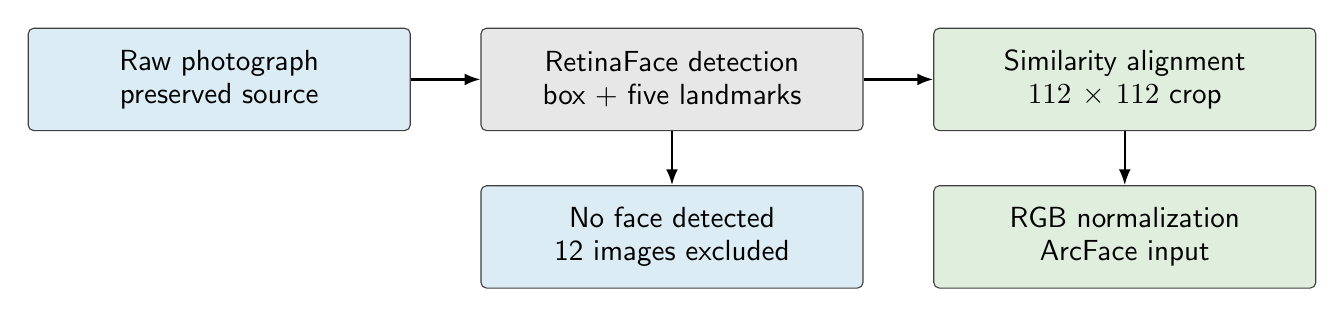
\begin{tikzpicture}
\node[box,fill=input] (raw) at (0,0) {Raw photograph\\preserved source};
\node[box,fill=frozen] (det) at (5.75,0) {RetinaFace detection\\box + five landmarks};
\node[box,fill=out] (crop) at (11.5,0) {Similarity alignment\\$112\times112$ crop};
\node[box,fill=input] (fail) at (5.75,-2) {No face detected\\12 images excluded};
\node[box,fill=out] (norm) at (11.5,-2) {RGB normalization\\ArcFace input};
\draw[arrow](raw)--(det);\draw[arrow](det)--(crop);
\draw[arrow](det)--(fail);\draw[arrow](crop)--(norm);
\end{tikzpicture}
\captionof{figure}{Fixed detector/alignment preprocessing. Detection failures remain outside the recognition manifest and all E0/E1/E2 query sets.}
\label{fig:preprocess}
\end{center}
\textbf{Duplicates and missing data.} There are 429 repeated MD5 occurrences beyond the first occurrence of each hash in the retained manifest. These records are retained, so this dataset must not be described as deduplicated. Missing detector outputs are excluded rather than imputed. All manifest cells are populated. Two additional DNG files mentioned in the technical report were not converted to JPEG; they are a format-handling issue outside the 6,000-image detection denominator.

\textbf{Leakage control.} Complete identities share one train/validation/test role within a fold. A clean photograph with maximal detection confidence supplies each person's fixed benchmark. That image and its associated burst neighbours are excluded from queries. Thus near-duplicate frames within a participant cannot cross the role boundary, and enrollment-related frames do not inflate query accuracy. Test-person benchmarks are legitimate enrollment data; their ordinary query images are absent from optimization.

\textbf{Training-only augmentation.} The final recipe applies horizontal flip ($p=0.5$), downscale/upscale blur ($0.3$), Gaussian blur ($0.15$), Gaussian pixel noise ($0.2$), JPEG quality 50--95 ($0.3$), and brightness/contrast jitter ($0.2$). Validation/test crops remain unaugmented. These transforms simulate capture variability, not new identities. The earlier report also discloses a small unflagged subset of digitally added coverings; its exact count and affected images are unknown. This provenance limitation is retained in Sections 12--13.
Figure~\ref{fig:det} describes detector confidence among the retained crops.
\fig{det_scores.pdf}{.74}{Detection confidence for the 5,988 retained face crops. Images with no detected face are absent from this distribution.}{fig:det}

% PAGE 9
\nextpage
\section{Technical Validation and Data Quality}
Table~\ref{tab:quality} separates data checks from recognition results. Figure~\ref{fig:detfail} shows five selected examples from the twelve raw photographs excluded after detection failure.
\begin{datatable}{Data-quality evidence and its limits.}{tab:quality}
\begin{tabularx}{\linewidth}{L{32mm}Y}\toprule
Quality dimension & Evidence / checks performed\\\midrule
Completeness & 5,988/6,000 detections (99.8\%); 13 populated fields; all 5,988 crops present\\
Consistency & 8 coverings, 2 lighting labels, 30 IDs; exclusions leave 5,818 queries\\
Label quality & Capture labels, manual quality review and completed inter-rater agreement checking; agreement method and coefficient: not supplied\\
Measurement quality & Fixed alignment; 12 detector failures; calibration details: not supplied\\
Integrity & Recorded hashes identify 429 duplicate occurrences\\
Representativeness / bias & Single-sitting convenience sample; scarf covers 24 people. Ages: 23--24 years (26 people); 28, 39, 44 and 78 years (one each). The collection is strongly concentrated in young adults.\\
Reproducibility & \codeurl; seed 42; saved folds/scripts/histories. Software versions: not supplied.\\\bottomrule
\end{tabularx}
\end{datatable}
\cont{RetinaFace failure cases: rejected raw photographs}
\fig{retinaface_rejected.pdf}{1}{RetinaFace rejection examples 1, 2, 5, 6 and 7 from the original twelve-image gallery, with original example numbers retained. These five photographs have no aligned crop or recognition prediction. The total measured detection-failure count remains twelve.}{fig:detfail}
\subsection{Comparison with Existing Datasets and Significance}
Table~\ref{tab:comparison} compares dataset properties. The studies in Section 5 use different tasks and sampling, so their published accuracies cannot be ranked directly against this experiment.
\begin{datatable}{Comparison with the closest supplied dataset precedent.}{tab:comparison}
\begin{tabularx}{\linewidth}{L{35mm}Y Y}\toprule
Property & Pgu-Face~\cite{pgu} & This dataset\\\midrule
Identities / images & 224 / 896 & 30 / 6,000 raw; 5,988 crops\\
Coverage & Facial-hair and sunglasses variation & Eight coverings; regular/low lighting\\
Capture structure & Up to two sessions, at least six days apart & One sitting per participant\\
ML artifacts & Dataset contribution & Fixed gallery, six folds, predictions and histories\\\bottomrule
\end{tabularx}
\end{datatable}
\begin{itemize}
\item More images per person and combined coverings support within-person occlusion analysis.
\item Fewer people and one-sitting capture limit claims about population or temporal diversity.
\end{itemize}

% PAGE 10
\nextpage
\section{Machine Learning (ML) Use Demonstration}
\subsection{ML task definition}
Given an aligned face crop $x$, identify its enrolled participant $y\in\{\mathrm{p01},\ldots,\mathrm{p30}\}$. All true query identities exist in the gallery, while validation/test identities are unseen during that fold's fine-tuning. The model returns the highest-scoring gallery identity if its cosine similarity is at least 0.3; otherwise it returns UNKNOWN. This is identification with a rejection option, not a test of stranger rejection.
\subsection{Data partitioning strategy}
Shuffle 30 people with seed 42 and divide them into six blocks of five. Fold $k$ uses block $k$ for testing, block $(k+1)\bmod6$ for validation, and the other four for training. Each person is tested once and validated once. Table~\ref{tab:folds} specifies the rotation; identities never share roles within a fold.
\begin{datatable}{Six-fold rotation. Training uses the remaining 20 identities in every row.}{tab:folds}
\begin{tabularx}{\linewidth}{L{12mm}Y Y}\toprule
Fold & Test identities & Validation identities\\\midrule
1 & p11, p15, p20, p23, p27 & p06, p07, p12, p13, p16\\
2 & p06, p07, p12, p13, p16 & p10, p17, p22, p26, p30\\
3 & p10, p17, p22, p26, p30 & p02, p03, p14, p19, p28\\
4 & p02, p03, p14, p19, p28 & p05, p08, p18, p25, p29\\
5 & p05, p08, p18, p25, p29 & p01, p04, p09, p21, p24\\
6 & p01, p04, p09, p21, p24 & p11, p15, p20, p23, p27\\\bottomrule
\end{tabularx}
\end{datatable}
The pooled test set contains 5,818 queries. Pooling uses exact counts, not an unweighted average of fold percentages. Test identities may be training identities in other folds, as expected in cross-validation, but their scored predictions come only from their held-out fold. Figures~\ref{fig:foldrotation} and \ref{fig:foldgrid} visualize the same six-fold split.
\begin{center}
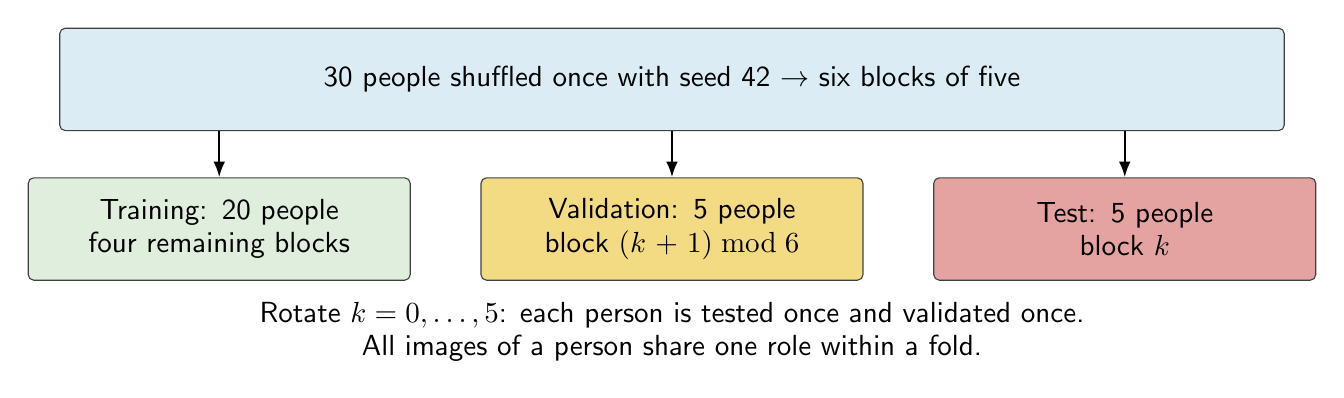
\begin{tikzpicture}
\node[box,fill=input,text width=152mm] (all) at (5.75,0) {30 people shuffled once with seed 42 $\to$ six blocks of five};
\node[box,fill=out] (tr) at (0,-1.9) {Training: 20 people\\four remaining blocks};
\node[box,fill=validation] (va) at (5.75,-1.9) {Validation: 5 people\\block $(k+1)\bmod6$};
\node[box,fill=rejected] (te) at (11.5,-1.9) {Test: 5 people\\block $k$};
\foreach \n in {tr,va,te}{\draw[arrow](all.south -| \n.north)--(\n.north);}
\node[font=\sffamily\fontsize{10.5}{12}\selectfont,align=center] at (5.75,-3.2) {Rotate $k=0,\ldots,5$: each person is tested once and validated once.\\All images of a person share one role within a fold.};
\end{tikzpicture}
\captionof{figure}{Six-fold person-disjoint rotation, following the technical report's split diagram. The formula uses zero-based block indices; Table~\ref{tab:folds} lists folds 1--6.}
\label{fig:foldrotation}
\end{center}
\nextpage
\cont{10.2 Data partitioning strategy (continued)}
\fig{fold_assignment.pdf}{1}{Full six-fold assignment grid regenerated from the saved fold JSON. Green = training, yellow = validation, red = testing. Each column contains four training roles, one validation role and one test role.}{fig:foldgrid}
\subsection{Preprocessing and feature/representation steps}
From each person's \code{none} images, select the photograph with maximal detector confidence, using no identity-query performance criterion. Extract one L2-normalized 512-dimensional benchmark with the original pretrained network. These 30 fixed vectors are shared across folds and experiments. Figure~\ref{fig:benchmark} distinguishes the training target set from the evaluation gallery.
\begin{center}
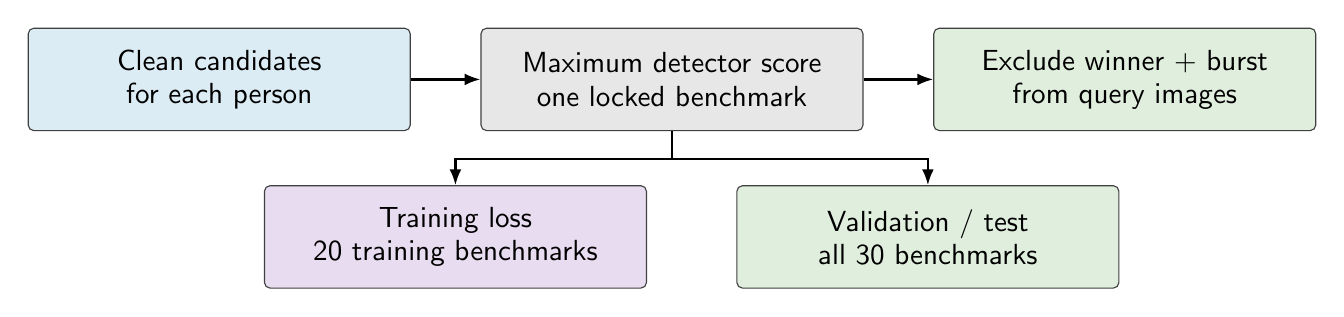
\begin{tikzpicture}
\node[box,fill=input] (a) at (0,0) {Clean candidates\\for each person};
\node[box,fill=frozen] (b) at (5.75,0) {Maximum detector score\\one locked benchmark};
\node[box,fill=out] (c) at (11.5,0) {Exclude winner + burst\\from query images};
\node[box,fill=train] (d) at (3,-2) {Training loss\\20 training benchmarks};
\node[box,fill=out] (e) at (9,-2) {Validation / test\\all 30 benchmarks};
\draw[arrow](a)--(b);\draw[arrow](b)--(c);
\draw[arrow](b.south)--++(0,-.35)-|(d.north);
\draw[arrow](b.south)--++(0,-.35)-|(e.north);
\end{tikzpicture}
\captionof{figure}{Benchmark preparation and use. Gallery vectors never enter the optimizer. The final embedding projection inside the backbone is a distinct component and is trainable only in E2.}
\label{fig:benchmark}
\end{center}

% PAGE 11
\nextpage
\subsection{ML model(s) and hyperparameters}
\cont{Full ArcFace / IResNet-50 architecture: input to output}
Figure~\ref{fig:fullarcface} shows the actual \code{w600k\_r50.onnx} network with its input and output dimensions; $N$ is the batch size. ArcFace is the angular-margin learning method, while IResNet-50 is the embedding backbone used here.
\begin{center}
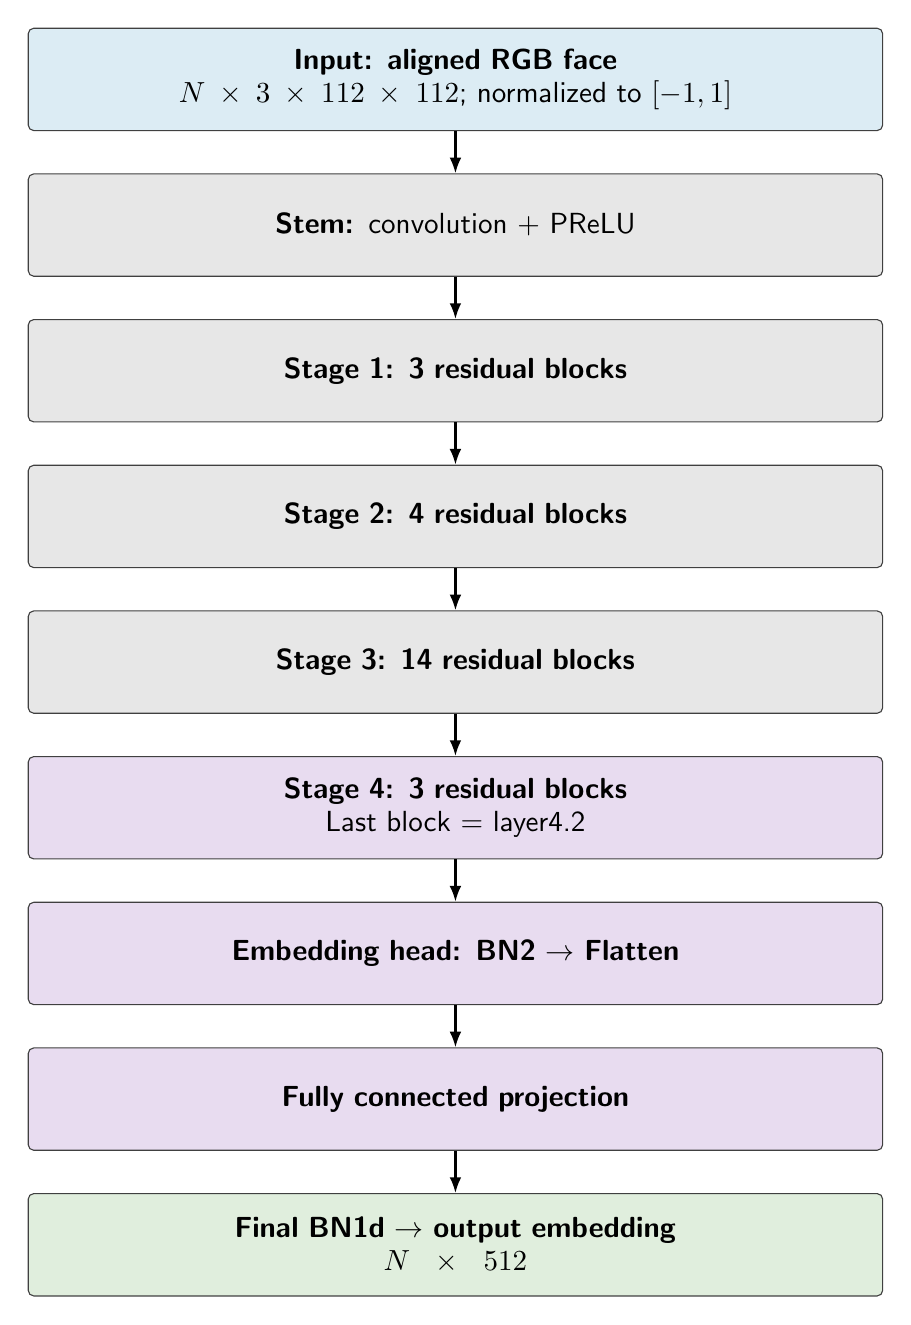
\begin{tikzpicture}[main/.style={box,text width=105mm}]
\node[main,fill=input] (in) at (0,0) {\textbf{Input: aligned RGB face}\\$N\times3\times112\times112$; normalized to $[-1,1]$};
\node[main,fill=frozen] (stem) at (0,-1.85) {\textbf{Stem:} convolution + PReLU};
\node[main,fill=frozen] (s1) at (0,-3.7) {\textbf{Stage 1: 3 residual blocks}};
\node[main,fill=frozen] (s2) at (0,-5.55) {\textbf{Stage 2: 4 residual blocks}};
\node[main,fill=frozen] (s3) at (0,-7.4) {\textbf{Stage 3: 14 residual blocks}};
\node[main,fill=train] (s4) at (0,-9.25) {\textbf{Stage 4: 3 residual blocks}\\Last block = layer4.2};
\node[main,fill=train] (flat) at (0,-11.1) {\textbf{Embedding head: BN2 $\to$ Flatten}};
\node[main,fill=train] (fc) at (0,-12.95) {\textbf{Fully connected projection}};
\node[main,fill=out] (outp) at (0,-14.8) {\textbf{Final BN1d $\to$ output embedding}\\$N\times512$};
\foreach \a/\b in {in/stem,stem/s1,s1/s2,s2/s3,s3/s4,s4/flat,flat/fc,fc/outp}{\draw[arrow](\a)--(\b);}

\end{tikzpicture}
\captionof{figure}{Complete ArcFace IResNet-50 architecture from aligned RGB input to the 512-dimensional output embedding. The four stages contain $[3,4,14,3]$ blocks. The following figure separately specifies the E0/E1/E2 update scopes.}
\label{fig:fullarcface}
\end{center}
The graph contains 43,590,976 parameters. Its output is a 512-dimensional embedding, not 30 class probabilities. Outside the ONNX backbone, the embedding is L2-normalized and matched by cosine similarity against the enrollment gallery, which supplies the candidate identities.
\nextpage
\cont{10.4 ML model(s) and hyperparameters (continued)}
\cont{ArcFace architecture and E0 / E1 / E2 experiments}
The ArcFace method~\cite{arcface} supplies the angular-margin objective. The \code{w600k\_r50.onnx} IResNet-50 graph contains 43,590,976 parameters, residual stages with $[3,4,14,3]$ blocks, and a 512-dimensional output. Figure~\ref{fig:architecture} shows each experimental architecture. Table~\ref{tab:scopes} names the exact unfrozen modules.
\begin{center}
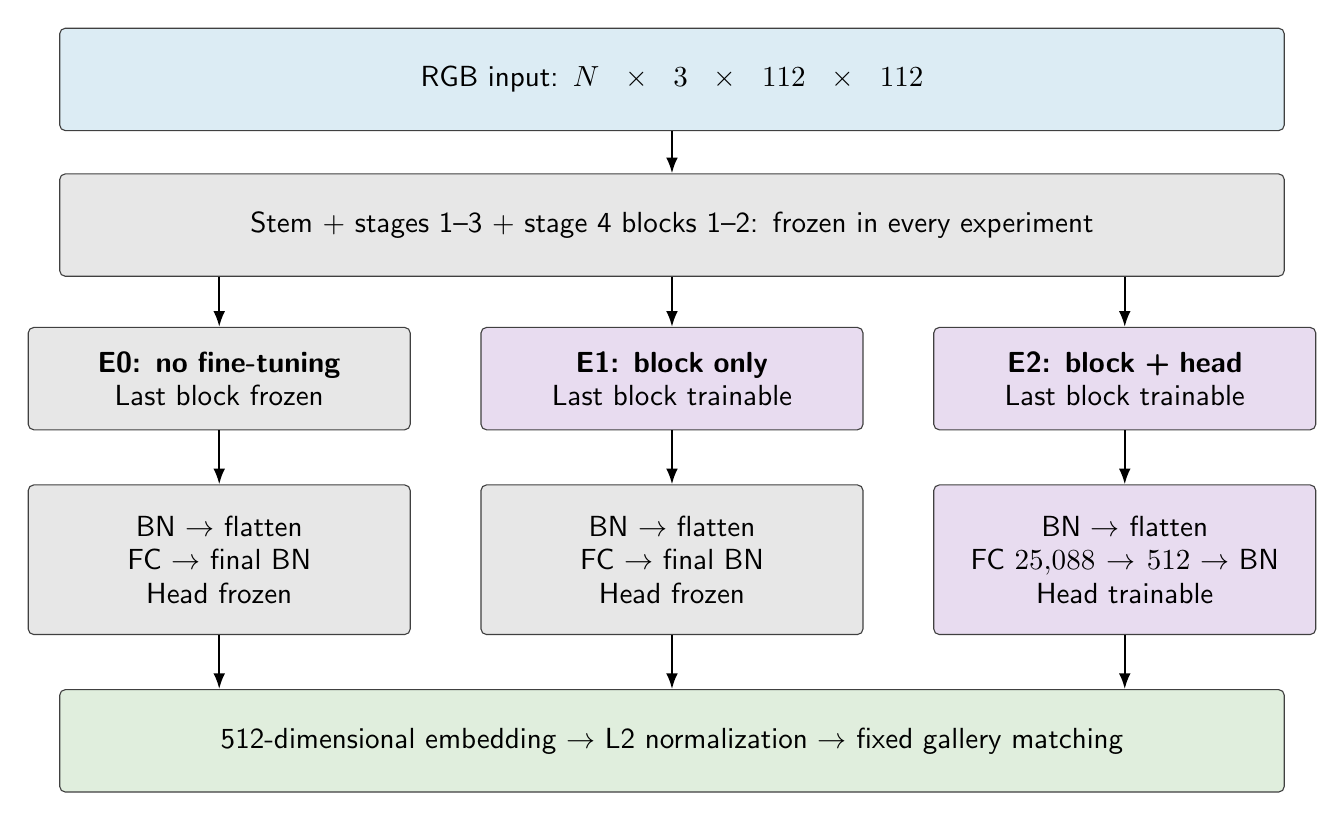
\begin{tikzpicture}
\node[box,fill=input,text width=152mm] (a) at (5.75,0) {RGB input: $N\times3\times112\times112$};
\node[box,fill=frozen,text width=152mm] (b) at (5.75,-1.85) {Stem + stages 1--3 + stage 4 blocks 1--2: frozen in every experiment};
\node[box,fill=frozen] (c0) at (0,-3.8) {\textbf{E0: no fine-tuning}\\Last block frozen};
\node[box,fill=train] (c1) at (5.75,-3.8) {\textbf{E1: block only}\\Last block trainable};
\node[box,fill=train] (c2) at (11.5,-3.8) {\textbf{E2: block + head}\\Last block trainable};
\node[box,fill=frozen,minimum height=19mm] (d0) at (0,-6.1) {BN $\to$ flatten\\FC $\to$ final BN\\Head frozen};
\node[box,fill=frozen,minimum height=19mm] (d1) at (5.75,-6.1) {BN $\to$ flatten\\FC $\to$ final BN\\Head frozen};
\node[box,fill=train,minimum height=19mm] (d2) at (11.5,-6.1) {BN $\to$ flatten\\FC $25{,}088\to512$ $\to$ BN\\Head trainable};
\node[box,fill=out,text width=152mm] (e) at (5.75,-8.4) {512-dimensional embedding $\to$ L2 normalization $\to$ fixed gallery matching};
\draw[arrow](a)--(b);
\foreach \i in {0,1,2}{\draw[arrow](b.south -| c\i.north)--(c\i.north);\draw[arrow](c\i)--(d\i);\draw[arrow](d\i.south)--(e.north -| d\i.south);}
\end{tikzpicture}
\captionof{figure}{E0, E1 and E2 architecture views. Gray = frozen; purple = trainable; blue = input; green = output. The last block is layer4.2. Flatten has no parameters, and all BN running statistics remain frozen.}
\label{fig:architecture}
\end{center}
\begin{datatable}{Experiment scopes. The gallery/training benchmark matrix remains fixed in all cases.}{tab:scopes}
\begin{tabularx}{\linewidth}{L{13mm}Y r}\toprule
Model & Unfrozen ONNX modules & Trainable parameters\\\midrule
E0 & None; original pretrained network & 0\\
E1 & BatchNormalization\_121, Conv\_122, Conv\_124 & 4,720,640\\
E2 & E1 plus BatchNormalization\_126, Gemm\_128, BatchNormalization\_129 & 17,568,256\\\bottomrule
\end{tabularx}
\end{datatable}
\nextpage
\cont{10.4 Model architectures (continued): RetinaFace detector}
The project's RetinaFace stage~\cite{retinaface}, \code{det\_10g.onnx}, is always frozen: 4,225,835 parameters and 158 ONNX nodes. Figure~\ref{fig:detarchitecture} shows its three-scale outputs; Table~\ref{tab:detector} summarizes what each output represents.
\begin{center}
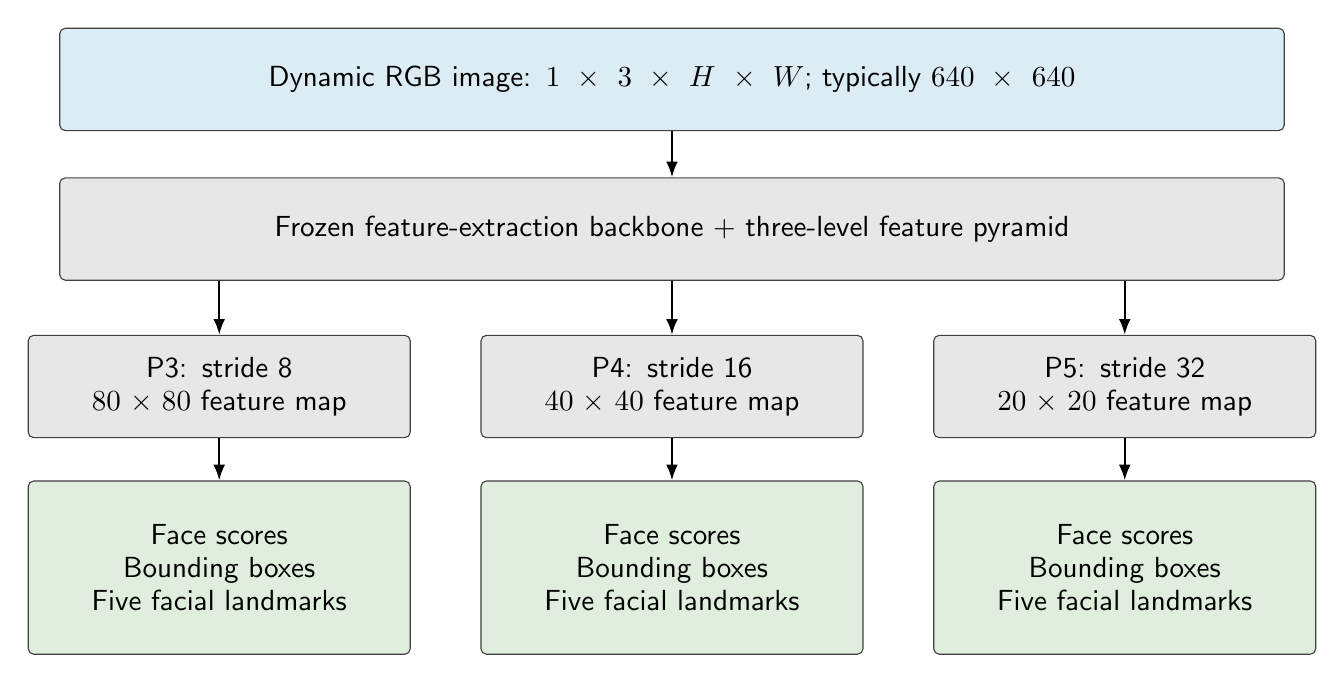
\begin{tikzpicture}
\node[box,fill=input,text width=152mm] (a) at (5.75,0) {Dynamic RGB image: $1\times3\times H\times W$; typically $640\times640$};
\node[box,fill=frozen,text width=152mm] (b) at (5.75,-1.9) {Frozen feature-extraction backbone + three-level feature pyramid};
\node[box,fill=frozen] (p3) at (0,-3.9) {P3: stride 8\\$80\times80$ feature map};
\node[box,fill=frozen] (p4) at (5.75,-3.9) {P4: stride 16\\$40\times40$ feature map};
\node[box,fill=frozen] (p5) at (11.5,-3.9) {P5: stride 32\\$20\times20$ feature map};
\node[box,fill=out,minimum height=22mm] (h3) at (0,-6.2) {Face scores\\Bounding boxes\\Five facial landmarks};
\node[box,fill=out,minimum height=22mm] (h4) at (5.75,-6.2) {Face scores\\Bounding boxes\\Five facial landmarks};
\node[box,fill=out,minimum height=22mm] (h5) at (11.5,-6.2) {Face scores\\Bounding boxes\\Five facial landmarks};
\draw[arrow](a)--(b);
\foreach \i in {3,4,5}{\draw[arrow](b.south -| p\i.north)--(p\i.north);\draw[arrow](p\i)--(h\i);}
\end{tikzpicture}
\captionof{figure}{RetinaFace detection architecture: three output scales, each with classification, box regression and landmark heads.}
\label{fig:detarchitecture}
\end{center}
\begin{datatable}{RetinaFace outputs at each of the three feature-pyramid levels.}{tab:detector}
\begin{tabularx}{\linewidth}{L{35mm}Y}\toprule
Output & Meaning\\\midrule
Face scores & Confidence that a candidate region contains a face\\
Bounding boxes & Face location and extent in the image\\
Five facial landmarks & Left eye, right eye, nose, left mouth corner and right mouth corner\\\bottomrule
\end{tabularx}
\end{datatable}

The facial landmarks drive the similarity transform before the recognizer receives an aligned crop. The detector remains fixed across E0, E1 and E2, so the adaptation comparison changes recognition rather than detection.

The analyzed ONNX graph includes 58 convolution, 36 ReLU, 16 addition, three average-pooling, three sigmoid, two resize and one max-pooling nodes, among its 158 total nodes. The three resolutions permit detection at different face scales. Nine output tensors result: score, box and landmark outputs for each of the three levels.

% PAGE 12
\nextpage
\cont{10.4 ML model(s) and hyperparameters (continued)}
\textbf{Locked targets and gradient updates.} An augmented training image produces a normalized embedding. Its cosine similarities to the 20 training-person benchmarks become logits. Only the true class receives the additive angular margin; all logits are scaled by 32 before cross-entropy with label smoothing 0.1. Figure~\ref{fig:training} shows the loss route. E1/E2 differ only in which backbone parameters the optimizer can update.
\begin{center}
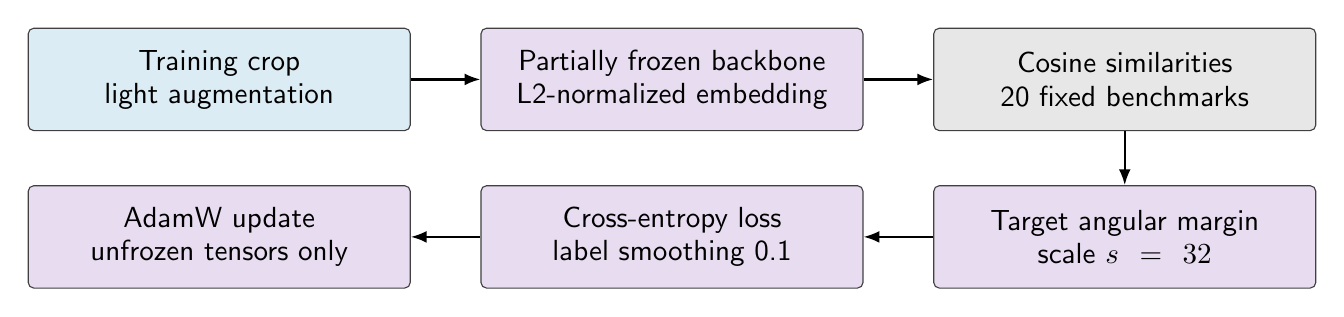
\begin{tikzpicture}
\node[box,fill=input] (a) at (0,0) {Training crop\\light augmentation};
\node[box,fill=train] (b) at (5.75,0) {Partially frozen backbone\\L2-normalized embedding};
\node[box,fill=frozen] (c) at (11.5,0) {Cosine similarities\\20 fixed benchmarks};
\node[box,fill=train] (d) at (11.5,-2) {Target angular margin\\scale $s=32$};
\node[box,fill=train] (e) at (5.75,-2) {Cross-entropy loss\\label smoothing 0.1};
\node[box,fill=train] (f) at (0,-2) {AdamW update\\unfrozen tensors only};
\draw[arrow](a)--(b);\draw[arrow](b)--(c);\draw[arrow](c)--(d);\draw[arrow](d)--(e);\draw[arrow](e)--(f);
\end{tikzpicture}
\captionof{figure}{Training forward/loss sequence. Gradients pass through the fixed embedding head in E1 to reach its trainable residual block; frozen parameters are not updated.}
\label{fig:training}
\end{center}
The true-class logit is $32\cos(\theta_y+m_t)$; other logits are $32\cos\theta_j$. Figure~\ref{fig:margin} shows the warmup and ramp, reaching full margin at epoch 6.
\begin{center}
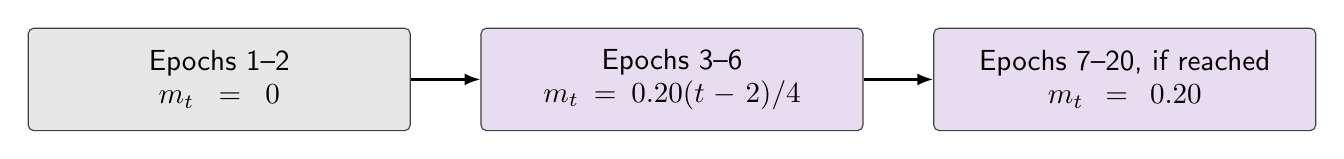
\begin{tikzpicture}
\node[box,fill=frozen] (a) at (0,0) {Epochs 1--2\\$m_t=0$};
\node[box,fill=train] (b) at (5.75,0) {Epochs 3--6\\$m_t=0.20(t-2)/4$};
\node[box,fill=train] (c) at (11.5,0) {Epochs 7--20, if reached\\$m_t=0.20$};
\draw[arrow](a)--(b);\draw[arrow](b)--(c);
\end{tikzpicture}
\captionof{figure}{Angular-margin schedule shared by E1 and E2. E0 executes no training updates.}
\label{fig:margin}
\end{center}
\begin{datatable}{Shared E1/E2 training settings. E0 performs zero training epochs.}{tab:hyper}
\begin{tabularx}{\linewidth}{L{55mm}Y}\toprule
Hyperparameter & Value\\\midrule
Optimizer / learning rate / weight decay & AdamW / $3\times10^{-5}$ / $10^{-4}$\\
Learning-rate schedule & Cosine annealing, $T_{\max}=20$\\
Train / evaluation batch size & 32 / 64\\
Maximum epochs / patience & 20 / 5 non-improving epochs\\
Full angular margin / logit scale & 0.20 / 32\\
Label smoothing / random seed & 0.1 / 42\\
Checkpoint criterion & Highest validation accepted-correct rate; ties broken by mean benchmark gap; strict improvement\\
Initial candidate & Epoch 0, the pretrained model before any update\\\bottomrule
\end{tabularx}
\end{datatable}
\textbf{Batch normalization.} Running means and variances stay frozen because the backbone remains in evaluation mode. Affine scale/shift parameters are trainable only where included in the unfreeze scope. A frozen layer can still transmit gradients to a preceding trainable layer.

\textbf{Model selection.} Validate against the full 30-person gallery after each epoch. If five successive epochs do not improve the ordered pair of validation accuracy and benchmark gap, stop. Keeping epoch 0 is valid; E2 does so in folds 3, 4 and 5. E1 selects epoch 5 in five folds and epoch 8 in fold 4. E2 has about 3.7 times E1's trainable capacity, primarily from its $512\times25{,}088$ fully connected matrix.

% PAGE 13
\nextpage
\subsection{Evaluation metrics}
For unit-normalized query $z$ and gallery vectors $g_j$, let $\hat y=\arg\max_j z^\top g_j$ and $s_{\max}=\max_j z^\top g_j$.
A query is correct exactly when $\hat y=y$ and $s_{\max}\ge0.3$. Accuracy is the number of such queries divided by all queries. Every rejection is a miss because all test people are enrolled. The four mutually exclusive outcomes are: accepted/correct; rejected with the right top identity; rejected with the wrong top identity; and accepted/wrong (misidentified).

Each confusion matrix has 30 true-identity rows and 31 predicted columns: 30 identities plus REJECT. For identity $i$, precision is $TP_i/(TP_i+FP_i)$, recall is $TP_i/(TP_i+FN_i)$, and $F1_i=2P_iR_i/(P_i+R_i)$. A rejection contributes a false negative for the true identity and no false positive for another identity. Macro metrics average the 30 identity-level values. Macro recall and pooled accuracy can differ because identity supports differ.

\cont{Inference and the acceptance / UNKNOWN threshold}
Figure~\ref{fig:inference} shows the complete inference route. The threshold remains 0.3; no stranger cohort is supplied, so open-set false-accept rates are not measured.
\begin{center}
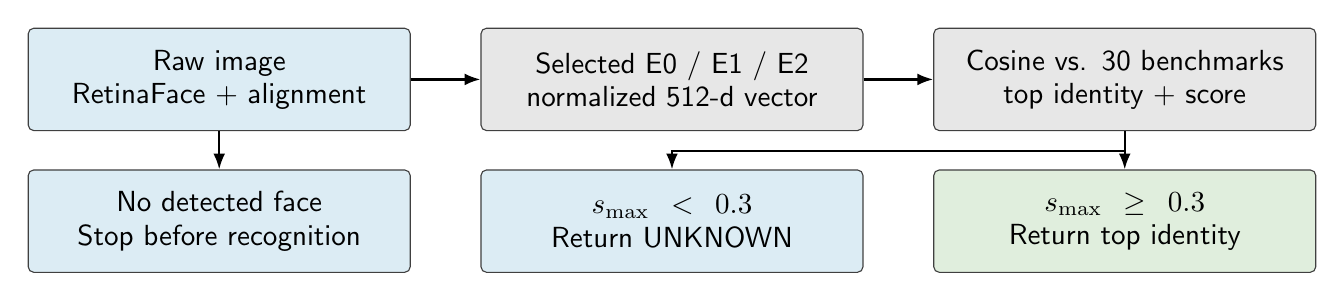
\begin{tikzpicture}
\node[box,fill=input] (a) at (0,0) {Raw image\\RetinaFace + alignment};
\node[box,fill=frozen] (b) at (5.75,0) {Selected E0 / E1 / E2\\normalized 512-d vector};
\node[box,fill=frozen] (c) at (11.5,0) {Cosine vs. 30 benchmarks\\top identity + score};
\node[box,fill=out] (d) at (11.5,-1.8) {$s_{\max}\ge0.3$\\Return top identity};
\node[box,fill=input] (e) at (5.75,-1.8) {$s_{\max}<0.3$\\Return UNKNOWN};
\node[box,fill=input] (f) at (0,-1.8) {No detected face\\Stop before recognition};
\draw[arrow](a)--(b);\draw[arrow](b)--(c);\draw[arrow](c)--(d);
\draw[arrow](c.south)--++(0,-.25)-|(e.north);\draw[arrow](a)--(f);
\end{tikzpicture}
\captionof{figure}{Inference uses no angular margin, label smoothing or weight update. Detection failure and low-similarity rejection are separate outcomes; an accepted identity can still be wrong.}
\label{fig:inference}
\end{center}
\subsection{Reproducibility}
The final source reports seed 42 for the fold shuffle and training randomness. Before fine-tuning, converted recognizer output is checked against ONNX Runtime on random inputs, requiring cosine similarity at least 0.999. The original results were produced on the GPU system; the later CPU prediction export can move one threshold-borderline image across 0.3. Tables in this report retain the original pooled GPU counts and explicitly distinguish confusion-derived artifacts.

\cont{Reproduction and file index}
Obtain the code from \codeurl\ and the dataset from \datasetlink. Follow \path{docs/FINAL_README.txt}, use the files in Table~\ref{tab:files}, then run the following sequence from \code{scripts/}. Exact environment versions and machine-specific paths must be resolved before retraining.
\begin{enumerate}[label=\arabic*.,itemsep=1pt]
\item \path{20_e1e2_person_folds.py}: prepare gallery, exclusions and folds.
\item \path{19_e1e2_person_finetune.py}: all six folds and E0/E1/E2; maximum epochs 0/20/20, acceptance threshold 0.3.
\item \path{21_e1e2_confusion.py} and \path{23_dump_predictions.py}: metrics and per-query outcomes for each experiment.
\item \path{25_e1e2_learning_curve.py}: repeat E1/E2 with validation loss added; \path{27_e1e2_matched_curve.py}: repeat again, scoring the training people with the validation rule for the Section 10.7 curves.
\item \path{22_e1e2_plots.py}, \path{24_report_figures.py}: original figures; \path{docs/build_final_figures.py}: this report's vector figures, with no retraining.
\end{enumerate}
\textbf{Loss comparability.} The optimized objective uses a 20-person head, angular margin, label smoothing and augmented crops, so its value is not comparable with a validation loss. The curves in Section 10.7 therefore report one common objective on both sides: clean crops, no margin, no label smoothing and cross-entropy over the 30-person gallery, measured on the training people and on the held-out validation people. Their separation is a genuine generalization gap. This measurement changes no training result; the repeated runs reproduce every selected epoch.

% PAGE 14
\nextpage
\subsection{Results (compact)}
Table~\ref{tab:overall} reports pooled accuracy and macro metrics. E1 improves accuracy by 1.20 percentage points over E0; E2 is 0.26 points below E0. Table~\ref{tab:outcomes} shows why acceptance alone is inadequate: E2 converts more failures into accepted wrong identities. The per-fold results in Table~\ref{tab:foldresults} establish the consistency of E1's gain.
\begin{datatable}{Pooled performance over 5,818 queries, all 30 identities tested once. Macro metrics are from the saved confusion-derived summary.}{tab:overall}
\begin{tabularx}{\linewidth}{Y r r r r}\toprule
Model & Accuracy & Macro precision & Macro recall & Macro F1\\\midrule
E0 & 84.98\% & 100.00\% & 85.12\% & 91.67\%\\
E1 & \textbf{86.18\%} & 99.72\% & \textbf{86.33\%} & \textbf{92.15\%}\\
E2 & 84.72\% & 96.43\% & 84.87\% & 89.85\%\\\bottomrule
\end{tabularx}
\end{datatable}
\begin{datatable}{Outcome breakdown from original GPU fold counts. Percentage rounding can prevent displayed rows from summing to exactly 100\%.}{tab:outcomes}
\begin{tabularx}{\linewidth}{L{14mm}Y Y Y Y}\toprule
Model & Accepted, correct & Rejected, right top identity & Rejected, wrong top identity & Accepted, wrong identity\\\midrule
E0 & 84.98\% & 12.50\% & 2.53\% & 0.00\%\\
E1 & 86.18\% & 8.47\% & 5.12\% & 0.22\%\\
E2 & 84.72\% & 7.24\% & 4.73\% & 3.32\%\\\bottomrule
\end{tabularx}
\end{datatable}
\begin{datatable}{Per-fold accepted-correct accuracy. Parentheses give the selected epoch; zero means no fine-tuned checkpoint displaced the pretrained model.}{tab:foldresults}
\begin{tabularx}{\linewidth}{Y r r r r}\toprule
Fold & Queries & E0 & E1 (epoch) & E2 (epoch)\\\midrule
1 & 974 & 84.39\% & 86.76\% (5) & 85.01\% (5)\\
2 & 985 & 80.71\% & 81.02\% (5) & 81.02\% (6)\\
3 & 965 & 88.60\% & 89.02\% (5) & 88.60\% (0)\\
4 & 973 & 80.47\% & 82.01\% (8) & 80.47\% (0)\\
5 & 960 & 90.83\% & 92.40\% (5) & 90.83\% (0)\\
6 & 961 & 85.02\% & 86.06\% (5) & 82.52\% (6)\\\bottomrule
\end{tabularx}
\end{datatable}
E1 improves test accuracy in all six folds. E2 selects a trained checkpoint in three folds, but improves test accuracy over E0 in only folds 1 and 2; fold 6 declines and the other three folds tie E0. This distinction resolves the final source's shorthand statement that E2 ``wins'' in three folds.

\cont{Discussion and conclusion}
The ranking is E1 $>$ E0 $>$ E2. Last-block adaptation transfers modestly to held-out identities; adapting the embedding projection is less reliable. E2's larger projection matrix offers a plausible capacity-related explanation, but the experiment does not isolate that mechanism causally. E1's main benefit is concentrated in mask plus sunglasses. A frozen pretrained recognizer remains a strong baseline for milder conditions. No population-level significance claim is made from correlated burst images.

% PAGE 15
\nextpage
\cont{10.7 Results (continued): occlusion sensitivity and training behaviour}
Table~\ref{tab:occlusion} shows the largest E1 gain under mask plus sunglasses. Figures~\ref{fig:e1loss}--\ref{fig:e2loss} plot one common loss on the training and validation people, one colour per fold. The per-occlusion chart and validation-accuracy curves appear in Appendix B (Figures~\ref{fig:occlusion} and \ref{fig:epochs}).
\begin{datatable}{Per-occlusion query accuracy, pooled from the final fold results.}{tab:occlusion}
\begin{tabularx}{\linewidth}{Y r r r r}\toprule
Occlusion & Queries & E0 & E1 & E2\\\midrule
None & 667 & 100.0\% & 99.4\% & 99.6\%\\
Clear glasses & 667 & 100.0\% & 99.0\% & 98.7\%\\
Sunglasses & 826 & 98.5\% & 99.2\% & 97.2\%\\
Scarf & 551 & 97.3\% & 94.9\% & 96.0\%\\
Cap & 751 & 95.5\% & 95.2\% & 94.3\%\\
Mask & 853 & 90.2\% & 89.9\% & 88.0\%\\
Mask + clear glasses & 726 & 68.5\% & 68.9\% & 66.7\%\\
Mask + sunglasses & 777 & 35.6\% & \textbf{47.2\%} & 42.7\%\\\bottomrule
\end{tabularx}
\end{datatable}
The per-occlusion gain is concentrated in the hardest combined covering. Scarf has fewer identities, and every measurement conditions on detection having succeeded. The following page shows the training trajectories at larger scale.
\nextpage
\cont{10.7 Results (continued): learning curves}
\fig{e1_loss.pdf}{1}{E1: one common gallery loss on the training people (solid) and the held-out validation people (dashed), all six folds. Stars mark the selected epoch, which is chosen by validation accuracy, not by loss. Both sides start together at epoch 0; the training loss then falls to about 0.001 while the validation loss rises and never returns to its epoch-0 value.}{fig:e1loss}
\fig{e2_loss.pdf}{1}{E2: the same measurement. The gap opens wider than in E1, with validation losses ending between 0.38 and 0.91, and three folds keep the pretrained model.}{fig:e2loss}
\textbf{Confusion matrices and macro metrics.} Table~\ref{tab:overall} reports macro scores; Appendix B gives every 30-person matrix. Rejections dominate E0/E1 errors; E2 also has more accepted wrong identities. The 11.6-point E1 gain under mask plus sunglasses drives its net benefit.

% PAGE 16
\nextpage
\section{Usage Notes and Reuse Potential}
Obtain the authorized dataset files from the \datasetlink. Load \code{manifest.csv} with a CSV reader and resolve image basenames within the participant crop directory. Remap the original training-machine paths. Read the fold JSON before constructing datasets, use its explicit person lists, and apply the recorded query exclusions. Load the same fixed 30-person gallery for every experiment.

For recognition studies, use the aligned crops and fixed RGB normalization. For detector studies, request access to raw photographs, including failures; retained crops alone cannot measure detector recall. Suitable reuse includes occlusion-conditioned retrieval, feature analysis, threshold sensitivity on enrolled people, and alternative partial fine-tuning scopes. A new unknown-person cohort is required for open-set rejection evaluation. Preserve subject grouping when extending the collection or comparing models.
\section{Limitations and Known Biases}
The 30-person convenience sample and single-sitting capture limit demographic, geographic and temporal generalization. Twenty-six participants are aged 23--24 years; ages 28, 39, 44 and 78 have only one participant each. Scarf appears for only 24 participants, and condition coverage is uneven. Burst correlation and 429 repeated MD5 occurrences reduce independence; image count is not an effective independent-sample count. Pose is not labeled, and regular/low lighting categories do not measure illumination quantitatively. Some synthetic content was added, including digitally added coverings; without per-image flags, a strictly real-only analysis cannot be reconstructed. The 12 detector failures are absent from recognition metrics, biasing those metrics toward detectable faces. All queries belong to enrolled identities, so rejection performance for strangers is unknown. These limitations constrain reuse and interpretation, even when the saved experiments can be inspected.
\section{Ethics, Privacy and Responsible Data Use}
Table~\ref{tab:ethics} records the documented conditions and remaining provenance gaps.
\begin{datatable}{Ethics and data-use record. Unreported approvals or permissions are not assumed.}{tab:ethics}
\begin{tabularx}{\linewidth}{L{40mm}Y}\toprule
Item & Documentation / constraint\\\midrule
Human participants / consent & Every participant signed consent before photography; participation was voluntary and withdrawable. All participants are adults (23--78 years). Approval body/protocol: not supplied.\\
Privacy / de-identification & Participant codes replace names, but faces remain identifiable. Raw images and identity mapping are restricted to the six members. Recognizable report/demo photographs require separate optional permission.\\
Web / social-media data & Not applicable; primary in-person collection.\\
Copyright / third-party data & Published works are attributed. Pretrained models originate from InsightFace; model redistribution terms must accompany any future release. No public dataset license is documented.\\
AI-generated / synthetic content & Some synthetic content was added, including digitally added coverings. Generation method and proportion: not supplied. Training also uses the explicit image augmentations in Section 8.\\\bottomrule
\end{tabularx}
\end{datatable}

% PAGE 17
\nextpage
\section{Data and Code Availability}
Table~\ref{tab:availability} records availability; identifiable images remain access-controlled.
\begin{datatable}{Availability record for this submission.}{tab:availability}
\begin{tabularx}{\linewidth}{L{44mm}Y}\toprule
Item & Details\\\midrule
Repository name & Project dataset on Google Drive: \datasetlink\\
Dataset DOI / persistent identifier & Not supplied\\
Direct dataset URL & \url{https://drive.google.com/drive/u/1/folders/1XN55OGpozy5Rhbs5QRFMatlCMTAo8sPu}\\
Access instructions & Open the Drive folder and request owner permission if prompted. Follow participant consent conditions.\\
Dataset license & Academic/non-commercial participant consent; no public release license supplied\\
Code / notebook URL & \codeurl; \code{scripts/} files listed in Section 10.6\\
Code version / commit / release & Not supplied\\
README \& environment & \path{docs/FINAL_README.txt} covers files, variables, setup and reuse. Exact dependency versions / lockfile: not supplied.\\\bottomrule
\end{tabularx}
\end{datatable}
\nextpage
\section{Student Contributions (CRediT-style)}
Each student captured and annotated their own five participants. Beyond this common collection role, Farhan Tahmid handles E1/E2 training, fine-tuning and training--evaluation pipeline checking; implementation, integration, metric analysis and documentation are distributed among the other members as detailed below. Contribution percentages are proportionally normalized to total 100\%. Evidence E1--E6 is indexed in \path{docs/CONTRIBUTIONS.md}; these are supporting project artifacts, not an independent authorship audit.
\begin{datatable}{Student contributions and shared evidence.}{tab:contributions}
\begin{tabularx}{\linewidth}{L{20mm}L{31mm}L{15mm}Y L{19mm}}\toprule
Roll & Student & Share (\%) & Main contributions & Evidence / files\\\midrule
2107031 & Adiba Tahsin & 17.50 & Capture protocol and quality-review coordination; label/age summaries; data dictionary and consent documentation & E1, E6\\
2107044 & Arafat Islam & 15.83 & E0 baseline implementation; RetinaFace crop/failure review; manifest schema and duplicate checks & E1, E3, E5\\
2107046 & Arman Rahman Rafi & 16.67 & Six-fold/gallery/exclusion preparation; trainable-scope configuration; training--evaluation pipeline integration and leakage checks & E2, E3, E4\\
2107047 & Dip Shekhor Datta & 15.83 & Validation-based checkpoint selection; prediction/metric analysis; confusion matrices and occlusion/rejection interpretation & E3, E4, E5\\
2107057 & Megha Tania & 16.67 & Learning-curve and architecture visualizations; base-paper comparison; report/README editing and reference checks & E5, E6\\
2107059 & Farhan Tahmid & 17.50 & E1/E2 model training and fine-tuning; training--evaluation pipeline checking & E3, E4\\\bottomrule
\end{tabularx}
\end{datatable}
\section{Acknowledgements, Funding and Competing Interests}
\subsection{Acknowledgements / Funding}
The report acknowledges the consenting participants and course instructors Dr. Muhammad Aminul Haque Akhand and Nabil Faiyaz Sadi. Funding declaration: not supplied.
\subsection{Declaration of Competing Interests}
Competing-interests declaration: not supplied.

% PAGE 18
\nextpage
\section{References}
\begingroup\setstretch{1}\small
\renewcommand{\section}[2]{}%
\begin{thebibliography}{9}
\bibitem{pgu} S. R. Salari and H. Rostami, ``Pgu-Face: A Dataset of Partially Covered Facial Images,'' \textit{Data in Brief}, vol. 9, pp. 288--291, 2016. DOI: \href{https://doi.org/10.1016/j.dib.2016.09.002}{10.1016/j.dib.2016.09.002}.
\bibitem{chong} L. W. J. Chong, S.-C. Chong and T.-S. Ong, ``Masked Face Recognition Using Support Vector Machine and Convolutional Neural Network,'' \textit{ICoICT}, pp. 270--274, 2022. DOI: \href{https://doi.org/10.1109/ICoICT55009.2022.9914874}{10.1109/ICoICT55009.2022.9914874}.
\bibitem{montero} D. Montero, M. Nieto, P. Leskovsky and N. Aginako, ``Boosting Masked Face Recognition with Multi-Task ArcFace,'' \textit{SITIS}, pp. 184--189, 2022. DOI: \href{https://doi.org/10.1109/SITIS57111.2022.00042}{10.1109/SITIS57111.2022.00042}.
\bibitem{arcface} J. Deng, J. Guo, N. Xue and S. Zafeiriou, ``ArcFace: Additive Angular Margin Loss for Deep Face Recognition,'' \textit{Proceedings of CVPR}, 2019.
\bibitem{retinaface} J. Deng, J. Guo, E. Ververas, I. Kotsia and S. Zafeiriou, ``RetinaFace: Single-Shot Multi-Level Face Localisation in the Wild,'' \textit{Proceedings of CVPR}, 2020.
\end{thebibliography}
\endgroup
\section*{Appendix A. Complete Data Dictionary (continued)}
The six principal fields are defined in Table~\ref{tab:dictionary}. Table~\ref{tab:dictionarymore} completes the 13-column manifest schema. All fields are populated in the supplied snapshot. Paths and labels should be validated before reuse; no imputation is defined.
\begin{datatable}{Remaining manifest fields and reuse semantics. Together with Table~\ref{tab:dictionary}, this covers every manifest column.}{tab:dictionarymore}
\begin{tabularx}{\linewidth}{L{30mm}L{20mm}Y}\toprule
Field & Type / unit & Meaning, coding and missing-value rule\\\midrule
\code{image\_path} & Text / path & Original image reference; training-machine absolute path. Required; remap to local raw directory.\\
\code{crop\_path} & Text / path & Aligned image reference; required. Crop basename resolves under the person directory.\\
\code{source\_stem} & Text & Original capture/source filename; required provenance link, e.g. IMG\_20260822\_114227.jpg.\\
\code{md5} & Text / hash & Recorded 32-character MD5; required. Repeated values are retained duplicate evidence, not a unique row key.\\
\code{split} & Text / category & Legacy train/val/test label; present but superseded by the six-fold JSON in the final experiment.\\
\code{det\_ok} & Boolean text & Detection status; True for retained rows. Failed detections are absent, not represented by blank rows.\\
\code{det\_stage} & Text / category & Successful detector pass; primary or loose in this snapshot. Required; 5,928 primary and 60 loose.\\\bottomrule
\end{tabularx}
\end{datatable}
\textbf{Relationships.} The fold JSON links identity lists, one benchmark photo per person and excluded query paths. Prediction CSVs link each evaluated query to its true identity, top gallery identity, similarity score and outcome. Confusion CSV rows are true identities; the final prediction column is REJECT. JSON metric summaries and histories derive from those evaluation/training records rather than adding new observations.
\section*{Appendix B. Optional Supporting Material}
\fig{quality_rejected.pdf}{.92}{Original capture-review rejection examples from the previous report, Section 5: blur, darkness, full coverage and bad framing. These illustrate review reasons, not an additional quantified exclusion set.}{fig:qcrejected}

% PAGE 19
\nextpage
\cont{B.1 E0 confusion matrix and rejected-photo examples}
Figure~\ref{fig:e0cm} shows errors concentrated in rejection. Figure~\ref{fig:arcfail} shows actual rejected crops, including correct and wrong top identities.
\fig{e0_confusion.pdf}{.94}{E0 confusion matrix, row-normalized over 5,818 queries. Identity labels 01--30 denote p01--p30; R is rejection below the threshold. Rejections explain recall below 100\% despite 100\% macro precision.}{fig:e0cm}
\fig{arcface_rejected.pdf}{1}{Actual E0 rejected photographs. Labels show true identity $>$ top identity and cosine score $s$. Top row: correct nearest identity but very low score. Bottom row: wrong nearest identity, still below 0.3. All twelve are rejected, not accepted misidentifications.}{fig:arcfail}

% PAGE 20
\nextpage
\cont{B.2 E1 confusion matrix and per-occlusion chart}
Figure~\ref{fig:e1cm} shows fewer rejections with rare accepted identity errors. Figure~\ref{fig:occlusion} visualizes the condition-level scores in the main results table.
\fig{e1_confusion.pdf}{1}{E1 confusion matrix, row-normalized. Last-block fine-tuning yields 86.18\% pooled accuracy and 92.15\% macro F1; the rejection column remains the dominant error source.}{fig:e1cm}
\fig{occlusion.pdf}{1}{Accepted-correct accuracy by covering. E1 gains 11.6 percentage points for mask plus sunglasses; gains are not uniform across the other conditions.}{fig:occlusion}

% PAGE 21
\nextpage
\cont{B.3 E2 confusion matrix and validation-accuracy curves}
Figure~\ref{fig:e2cm} shows more accepted wrong identities. Figure~\ref{fig:epochs} compares the validation-accuracy trajectories and selected checkpoints.
\fig{e2_confusion.pdf}{1}{E2 confusion matrix, row-normalized. Macro precision falls to 96.43\%, and original GPU results report 3.32\% accepted misidentification. Folds 3, 4 and 5 retain the pretrained epoch-0 checkpoint.}{fig:e2cm}
\fig{epochs.pdf}{1}{Validation accepted-correct accuracy by epoch for E1 and E2. One line per fold; dots mark selected checkpoints. E2 selects epoch 0 in folds 3, 4 and 5. Both loss plots are in the main report, Section 10.7.}{fig:epochs}

% PAGE 22
\nextpage
\section*{Appendix C. Dataset Release and FAIR-Readiness Checklist}
Table~\ref{tab:fair} assesses the evidence supplied with this project. ``No'' denotes incomplete or unverified release readiness, not proof that the activity never occurred. Local availability alone does not establish a public, reusable release.
\begin{datatable}{Dataset release and FAIR-readiness checklist, following the supplied template.}{tab:fair}
\begin{tabularx}{\linewidth}{L{31mm}Y L{12mm}Y}\toprule
Checklist item & Criterion & Yes/No & Evidence / note\\\midrule
Findable & Repository URL; meaningful names; searchable metadata & Yes & Dataset and code URLs supplied; meaningful filenames and CSV metadata exist.\\
Accessible & Working access instructions and justified restrictions & No & Drive folder and permission-request route supplied; access permissions not independently tested. Consent restrictions apply.\\
Interoperable & Common formats; documented labels and schema & Yes & JPEG, CSV and JSON with fields documented in Section 7 and Appendix A. Model binaries require their frameworks.\\
Reusable & Explicit license, README, provenance, limitations and citation & No & README, citation guidance, provenance and limitations supplied; public redistribution license: not supplied. Consent restrictions apply.\\
Raw + processed separation & Original observations preserved separately from derived data & Yes & Source scripts and reports distinguish raw \code{processed\_data/} from aligned \code{crops/}.\\
Versioning & Version/date and change history recorded & Yes & Dataset version 1; submission 22/09/2026; documentation change record in \path{docs/FINAL_README.txt}.\\
Integrity & Duplicate/corruption/schema checks; useful checksums & No & Hashes, duplicate count and populated fields available; a complete raw-file checksum/corruption audit is not supplied.\\
Leakage safety & Related subjects/augmentations stay within partitions & Yes & Six-fold identity roles; benchmark and burst exclusions; training-only augmentation.\\
Reproducible processing & Code recreates processed data and baseline from released inputs & No & Scripts and histories exist, but exact environment and full authorized raw-data release are not supplied.\\
Ethics/privacy & Consent/approval/licensing requirements satisfied & No & Signed consent and access controls reported; approval details and complete release permissions are not independently available.\\
Documentation & README covers files, variables, setup and reuse & Yes & \path{docs/FINAL_README.txt} covers the file structure, 13 metadata fields, setup, reproduction and reuse precautions.\\
Team accountability & All six students' contributions recorded & Yes & Section 15 and \path{docs/CONTRIBUTIONS.md}: individual tasks, names/rolls, declared figures and evidence links.\\\bottomrule
\end{tabularx}
\end{datatable}
\textbf{Evidence hierarchy for this report.} Experiment definitions, model scopes, split rules and metrics follow the final technical report and its saved results. The prior report supplies submission details, base papers, participant recruitment, consent, capture categories and historical quality control. Its earlier experiment labels and image-level split results are superseded. Additional manifest checks and redrawn plots use the supplied local records; no recognition model was retrained for this document.
\end{document}
